\chapter{Foundations of digital forensics}
First of all, lets define what can be considered digital evidence.
There are many definition but the one that is most commonly used,and
the preferred one at the exam, is:
\begin{boxH}
  \textbf{Digital evidence} is \textit{any} information of evidential
  value whether memorized or sent in a \textbf{digital format}.
  \label{boxH:digital-evidence}
\end{boxH}
Digital evidence has some defining characteristics: it is invisible to
the untrained eye (it usually not simple to find), it may need to be
interpreted by a specialist, it may be altered or destroyed trough
normal use and it can be copied without limits (you must always work
on a copy to avoid tampering evidence).

Digital evidence, to be admissible in court, must have some
properties:
\begin{itemize}
  \item \textbf{Authenticity}: avoid any digital evidence
    \textbf{tampering}. Only certified formats should be used.
  \item \textbf{Reliable and believable}: the evidence must be redly
    \textbf{understandable} to the judge. Sometimes a report is not
    available to explain the evidence, so it must be self-explanatory.
  \item \textbf{Proportional}: \textbf{respect} fundamental
    \textbf{rights} of parties affected by the measure
  \item \textbf{Admissible}: \textbf{compliant with law} and best
    practices(admissible in court). One thing is to have evidence, the
    other is to have it admissible in court, and that's not always the
    case.
\end{itemize}

There are three main kinds of digital evidence:
\begin{itemize}
  \item \textbf{Created by man}: any piece of digital data that is the
    result of a step or action taken by a human person. Of those,
    there are two types:
    \begin{itemize}
      \item \textbf{Human to human}, such as an email
      \item \textbf{Human to machine}, such as a file saved on a disk
    \end{itemize}
  \item \textbf{Created independently by the computer}: any piece of
    digital data that is the result of the processing of data carried
    out by a software in accordance with a specific algorithm and
    without human intervention (e.g. telephone records or Internet
    Service Provider logs)
  \item \textbf{Created by both man and the computer}: an electronic
    spreadsheet where data is entered by the human, while the computer
    works out the result.
\end{itemize}

Lets now define what digital forensics is:
\begin{boxH}
  \textbf{Digital forensics} is the process of getting hold of
  evidence without modifying the IT system in which the evidence is
  found, ensure that the evidence acquired in another medium is
  identical to the original and analyze the evidence without modifying 
  it.
\end{boxH}

\subsubsection{The "Big Five" of digital forensics}
There are some principle that are to be followed during digital
forensics:
\begin{itemize}
  \item \textbf{Data Integrity}: No action taken should change
    electronic devices or media, which may subsequently be relied upon
    in court. 
  \item \textbf{Chain of Custody}: An audit trail of all actions taken
    when handling electronic evidence should be created and preserved. 
  \item \textbf{Specialist Support} If investigations involving search
    and seizure of electronic evidence it may be necessary to consult
    external specialists. 
  \item \textbf{Appropriate Training}: First responders must be
    appropriately trained to be able to search for and seize
    electronic evidence if no experts are available at the scene. 
  \item \textbf{Legality}: The person and agency in charge of the case
    are responsible for ensuring that the law and the above listed
    principles are adhered to. 
\end{itemize}

\section{Digital Investigation Procedure}
Digital investigation is carried out in many steps.
\subsection{Identify the Suspect}
The first phase is also the most difficult one, because there are many
tools to be anonymous in the internet.
The general approach to this phase is the following:
\begin{enumerate}
  \item An investigator receives a \textbf{complaint} by a victim of
    \textbf{cybercrime} or detect an illegal content on line. (OSINT
    can be used to detect illegal content)
  \item The investigator uses the Court System to compel the ISP to
    \textbf{reveal} a \textbf{physical location} that corresponds
    likely to the source of Network (\textbf{IP Address})
  \item Under a \textbf{warrant} (depending from the Jurisdiction) the location
    is searched and any computer or other device is seized
\end{enumerate}

But why the ISP has to cooperate and give away the IP address?
In the EU it is because \textbf{Data Retention Directive} 2006/24/EC,
that requires that all the data of the communication must be stored
for a certain amount of time, from 6 to 24 months. This directive was
unconstitutional in many countries,
\begin{boxH}
  \textbf{Data retention} (or data preservation) generally refers to
  the \textbf{storage} of call detail records (CDRs) of telephony and
  internet traffic and transaction data (IPDRs) by governments and
  commercial organizations
\end{boxH}
In any case data retention is usually a problem because there's no a
homogeneous law for data retention, mainly for privacy reasons.

Even if there's no data retention law, the request of user data
disclosure have been a lot in the past years have steadily increased,
because the processes have been automated, as you can also see from
figure \ref{fig:disclosure-req}.

\begin{figure}[H]
  \centering
  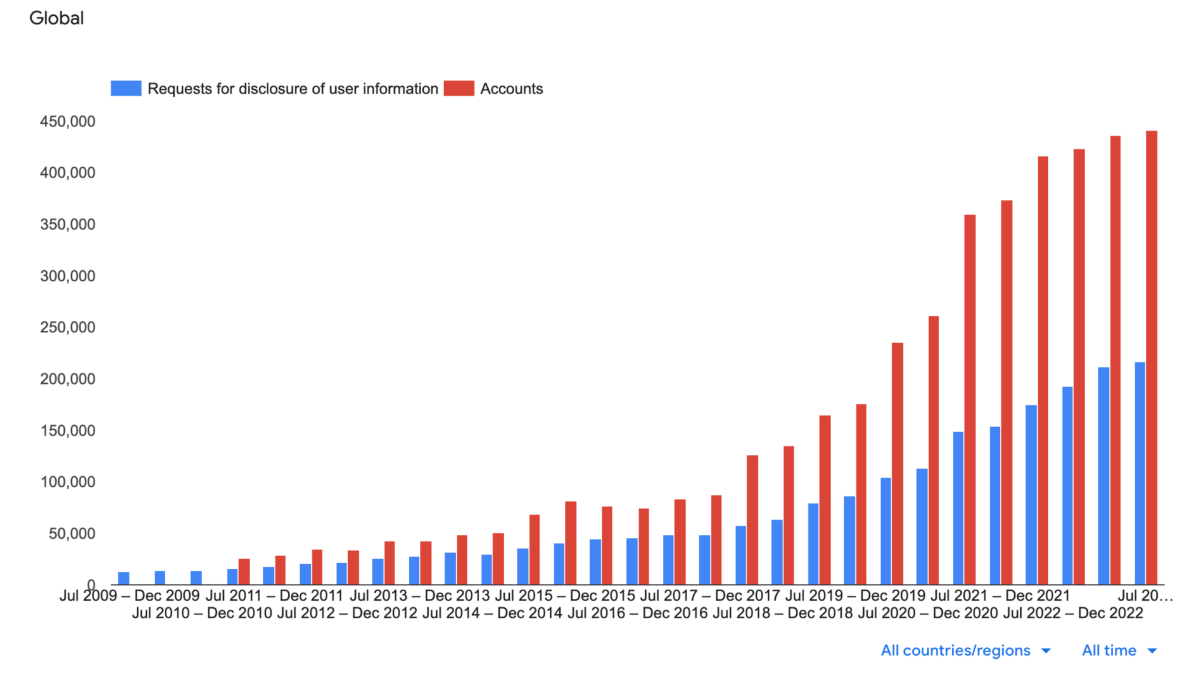
\includegraphics[scale=.4]{img/disclosure requests.png}
  \caption{Requests for user data disclosure during the years}
  \label{fig:disclosure-req}
\end{figure}
Another instrument that could be used to identify the suspect is the
\textbf{facial recognition}, that can be used only for terrorism
situations, but not in a systematic way.
\subsection{Detecting and Seizing Digital Evidence}
Anyone wanting to seize and validate digital/electronic evidences
(content of an e-mail or an entire hard-disk) has to respect two
fundamental \textbf{rules}: Bit-Stream Copy and Hash Function.
\subsubsection{Bit-Stream Copy}
\begin{boxH}
  A \textbf{bit-stream copy} can \textbf{clone} the \textbf{entire
  drive}.
\end{boxH}
It is a particular form of duplication in which the content of the
physical unit is read sequentially loading the minimum quantity of
data that can from time to time be directed, then recording it in the
same sequence on a standard binary file, generating a physical image
of the original medium.

\subsubsection{Hash Functions}
During the forensic analysis of modifiable media, the Hash 
guarantees the intangible nature of the data that it contains.
\begin{boxH}
  The Hash is a \textbf{one-way function}, by means of which a
  document of random length is converted into a limited and fixed
  length string.
\end{boxH}
This string represents a sort of ‘digital fingerprint’ of the non-
encrypted text, and is called the Hash Value or the Message Digest. If
the document is modified, even to the slightest extent, then the
fingerprint changes as well. In other words, by calculating and
recording the fingerprint, and then recalculating it, it can be shown
beyond all doubt whether the contents of the file, or the medium, have
been altered, even accidentally.\\

In any case we have two main problems while acquiring data: encryption
and jurisdiction. After all, the ISP, TELECO or even a bank does have
to cooperate and give out the data. Another big issue it the cloud
computing aspect, because the location of data is another big problem,
because it can be either:
\begin{itemize}
  \item \textbf{at rest}: does not reside on the device. 
  \item \textbf{in transit}: cannot be easily analysed because of
    encryption. 
  \item \textbf{in execution}: will be present only in the cloud
    instance
\end{itemize}
\textbf{Validation} of digital evidence is a very important step,
because it is the only way to prove that the evidence is authentic.
This is especially important for proof found on the internet. There
are some tools that can be used to validate digital evidence, such as
Web Forensics.\\
Another issue that has to be accouted for is the \textbf{chain of
custody}, that is the process of maintaining and documenting the
location and handling of evidence. After all, the bit is eternal, but
the storage medium is not.
\subsection{Validating Digital Evidence}
\subsection{Chain of Custody}
\subsection{Analysis of Digital Evidence}
\subsection{Presentation in Court}
